\documentclass[letterpaper]{article}
\IfFileExists{spanish.ldf}{%
  \usepackage[spanish,es-nodecimaldot]{babel}%
}{%
  \usepackage[provide=*,spanish]{babel}%
}
\selectlanguage{spanish}
\usepackage[utf8]{inputenc}
\usepackage[T1]{fontenc}
\usepackage{lmodern}
\usepackage{icomma}
\usepackage{microtype}
\usepackage{tabularx}
\setlength{\intextsep}{8pt plus 2pt minus 2pt}
\setlength{\abovecaptionskip}{6pt}
\clubpenalty=10000
\widowpenalty=10000

\usepackage{lipsum}
\usepackage{amsmath,amssymb,amsfonts,amsbsy}
\usepackage{array}
\usepackage{graphicx}
\usepackage{subfigure}
\usepackage{float}
\usepackage[hidelinks]{hyperref}
\def\UrlBreaks{\do\/\do-\do_\do.\do=\do?\do\&}

\graphicspath{ {./figures/} }

\usepackage[left=1.25in,right=1.25in,top=1.0in,bottom=1.0in]{geometry}
\usepackage{listings}

\usepackage{color}
\definecolor{deepblue}{rgb}{0,0,0.65}
\definecolor{deepred}{rgb}{0.7,0,0}
\definecolor{deepgreen}{rgb}{0,0.6,0}

\newcommand{\mytitle}{Tarea 1}
\newcommand{\myauthor}{Mariana Ortega}
\newcommand{\mydate}{\today}

\begin{document}

\noindent\begin{minipage}[t]{.13\textwidth}
	\vspace{-0.25in}
	\begin{figure}[H]
	
\includegraphics[width=0.90\textwidth]{LogoUC.jpg}
	\end{figure}
\end{minipage}
\hfill
\begin{minipage}[t]{.85\textwidth}
    \vspace{0pt}
    \begin{flushleft}
      \begin{tabular}{l}
	{\sc Pontificia Universidad Cat\'olica de Chile}\\
  	{\sc Escuela de Ingenier\'ia}\\
  	{\sc Departamento de Ingenier\'ia Industrial y Sistemas}\\
 	 {\sc ICS1113-Optimizaci\'on}
 \end{tabular}
	\end{flushleft}
\end{minipage}
\vspace{0pt}
\hfill
\vspace*{6cm}
\begin{center}{}
\vspace*{2mm}
{\Huge\bf Informe 4}\\
\vspace*{4mm}
\hrule\vspace*{1pt}\hrule
\vspace*{4mm}
{\LARGE\bf Red de recolecci\'on y valorizaci\'on de neum\'aticos fuera de uso bajo la Ley REP}\\
\vspace*{4mm}
{\huge\bf Grupo 52 }\\
\vspace*{1mm}
\end{center}

\vspace*{30mm}
\begin{flushright}
	
Vicente Baltra - 26646242 - 4 \\
Xavier Cacho - 24642193 - 3 \\
Nicolas Lenz - 25643010 - 3 \\
Raimundo Manríquez - 26646730 - 4 \\
Jorge Matamala - 20204124 - 1 \\
Fernanda Oyarzún - 24644064 - 1 \\
Vicente Villarroel - 25645455 - 3 \\

\vspace*{5mm}
{\large Fecha entrega: 13 de 11 de 2026\\}
\end{flushright}
\thispagestyle{empty}
\newpage

\thispagestyle{empty}
\renewcommand{\contentsname}{Índice}
\tableofcontents


\newpage
\pagenumbering{arabic}
\section{Introducción}

\subsection*{Contexto del problema}

Desde 2026, cuando alguien compra neumáticos nuevos en Chile, el comercializador queda obligado a recibir sin costo una cantidad equivalente de neumáticos usados~\cite{DS8}. Detrás de esa obligación hay una red completa que se encarga de retirar esos neumáticos y llevarlos a plantas donde se procesan mediante recauchaje, reciclaje material, coprocesamiento o valorización energética~\cite{DS8}, evitando que terminen en vertederos o basurales clandestinos.

Esa red la organizan entidades llamadas sistemas de gestión, que reúnen a distintas marcas de neumáticos y coordinan tanto la recolección como el procesamiento posterior. El más grande de estos en Chile es Valora Más~\cite{paiscircular2026}, que debe licitar de forma abierta los servicios de recolección y tratamiento~\cite{DS8}: por un lado busca empresas que recolecten los neumáticos en desuso de una región, y por otro, empresas gestoras que los valoricen en plantas autorizadas.

Este sistema se encuentra determinado por la Ley de Responsabilidad Extendida del Productor (Ley REP)~\cite{leyrep20920} y su reglamento (DS8)~\cite{DS8}, que establecen metas crecientes de recolección y valorización de neumáticos fuera de uso (NFU) para las marcas que venden estos productos. Las metas parten bajas en los primeros años de implementación de la ley y suben progresivamente hasta 2030, año en que tanto la meta de recolección como la de valorización alcanzan el 90\%~\cite{DS8,induambiente2021}. Este año 2026, las metas para neumáticos categoría A (aro inferior a 57 pulgadas, con excepción de los de aro igual a 45, 49 y 51 pulgadas) aumentaron de un 50\% a un 80\% en recolección y de un 35\% a un 60\% en valorización, medidas sobre los neumáticos puestos en el mercado el año anterior~\cite{DS8,paiscircular2026}, lo que ha generado una mayor dificultad en el cumplimiento de la ley respecto a los años anteriores.

\subsection*{Por qué es un problema}

El sistema licitatorio de Valora Más enfrenta dificultades para cubrir las regiones más extremas del país. En ellas hay pocos actores y no existen plantas de valorización, por lo que el material debe trasladarse hacia plantas del centro del país o exportarse~\cite{paiscircular2026}. En 2025 el sistema logró contar con servicios de recolección y valorización en al menos una ciudad o capital de cada región~\cite{paiscircular2025}, pero no alcanzó a cumplir la meta regional de recolección en las regiones más extremas~\cite{paiscircular2026}.

Desde 2025 las metas de la Ley REP se exigen además por región y no solo a nivel país~\cite{DS8}, así que esta desigualdad de cobertura deja de ser un tema secundario y pasa a ser un incumplimiento normativo directo si no se resuelve. El decreto fija un mínimo de recolección por región, expresado como porcentaje del total nacional de neumáticos puestos en el mercado el año anterior, ajustado por un factor de desgaste. Estos porcentajes son 15,3\% para la Región Metropolitana y, para el resto del país, 0,7\% en Arica y Parinacota; 1,2\% en Tarapacá; 2,4\% en Antofagasta; 2,5\% en Atacama; 2,1\% en Coquimbo; 4,7\% en Valparaíso; 3,5\% en O'Higgins; 4,2\% en Maule; 1,6\% en Ñuble; 4,2\% en Biobío; 2,6\% en Araucanía; 1,1\% en Los Ríos; 2,7\% en Los Lagos; 0,5\% en Aysén y 0,7\% en Magallanes~\cite{DS8}. En conjunto, estas cuotas regionales suman el 50\% de ese total nacional.

\subsection*{El problema de decisión}

Este es un problema de gestión, planificación y operación de un sistema de manejo de residuos urbanos, ya que los neumáticos fuera de uso se generan en las ciudades de todo el país y son uno de los productos prioritarios de la Ley REP~\cite{leyrep20920}. El desafío surge de compatibilizar dos objetivos que pueden entrar en conflicto: cumplir las metas nacionales y las cuotas regionales que exige la Ley REP y, al mismo tiempo, mantener una red de recolección y valorización que sea económicamente viable de operar. Frente a esto, Valora Más enfrenta la decisión de dónde ubicar sus centros de acopio y sus plantas de valorización, en qué momento habilitar cada uno dentro de su horizonte de planificación, qué tecnología de valorización usar en cada planta y cómo movilizar los neumáticos entre regiones, centros y plantas, de manera de cumplir las metas al menor costo posible. Este trabajo se acota a los neumáticos de categoría A, que concentran cerca del 78\% de los NFU~\cite{kyklos2026} y para los cuales se estiman las metas y la base del sistema en la justificación.

\section{Justificación}

\subsection*{Entidad beneficiada y valor de la solución}

La solución de este problema beneficia directamente a los sistemas de gestión colectivos de neumáticos, como Valora Más, que son quienes deben cumplir las metas nacionales y regionales de la Ley REP y hoy no cuentan con una forma sistemática de decidir dónde y cuándo instalar su infraestructura de recolección y valorización. Contar con este modelo les permite decidir en conjunto dónde ubicar los centros de acopio y las plantas de valorización, y no región por región como se hace hoy mediante licitaciones separadas, considerando en conjunto los efectos sobre los costos de transporte, operación y capacidad de la red.

\subsection*{Impacto cualitativo}

Más allá del costo, el problema tiene un componente de equidad territorial: las regiones más extremas y menos pobladas carecen de plantas de valorización y de mercados locales, por lo que sus neumáticos solo pueden valorizarse trasladándolos hacia el centro del país o exportándolos~\cite{paiscircular2026}. Antes de la Ley REP, solo cerca del 17\% de los neumáticos fuera de uso se manejaba de forma ambientalmente racional, y una fracción terminaba en basurales y vertederos clandestinos~\cite{DS8}. Una red diseñada para cumplir las cuotas regionales reduce la acumulación, el abandono y la quema informal de neumáticos, con los riesgos sanitarios y de incendio asociados, y permite que los habitantes de las regiones periféricas accedan al mismo servicio ambiental que el resto del país. El análisis económico y social que respalda el decreto estimó que sus beneficios superan 1,66 veces sus costos~\cite{DS8}, y un modelo que cumple las metas al menor costo contribuye directamente a que ese balance se materialice.

\subsection*{Impacto cuantitativo}

Según la gerenta general de Valora Más, en 2025 el sistema cumplió las metas nacionales de recolección y valorización, pero a la meta de recolección regional le faltaron algunos kilos, principalmente en las regiones más extremas~\cite{paiscircular2026}. La brecha de 2025 fue por lo tanto pequeña, pero el salto de 2026 y la ausencia de plantas en esas regiones la hacen crecer. Con una línea base de 189.000 toneladas de NFU en 2025, ya aplicado el factor de desgaste, de las cuales cerca del 78\% es categoría A, y con Valora Más agrupando a los productores del 52\% de esa categoría~\cite{kyklos2026}, la base del sistema es de cerca de 77.000 toneladas anuales. En 2026 esto equivale a metas de unas 61.000 toneladas de recolección y 46.000 de valorización. Las cuotas regionales, que suman el 50\% de esa base (unas 38.000 toneladas), exigen por ejemplo cerca de 380 toneladas anuales en Aysén y 540 en Magallanes~\cite{DS8}. Todas estas cifras son una estimación propia a partir de las fuentes citadas.

La brecha de 2025 no está cuantificada públicamente. Las cuotas de Arica y Parinacota, Aysén y Magallanes suman cerca de 1.460 toneladas anuales, un 1,9\% de la base. Como referencia, repartir el tope de 5.000 UTA por infracción grave~\cite{leyrep20920}, unos 4.300 millones de pesos con la UTA de octubre de 2026~\cite{sii2026}, entre ese volumen daría cerca de 2,9 millones de pesos por tonelada. Esta comparación ilustra la relevancia económica del incumplimiento; no constituye una tarifa legal por tonelada ni determina la sanción aplicable.


\section{Detalle del problema}

\subsection{Tomador de decisiones y objetivo}

El tomador de decisiones es Valora Más, el mayor sistema de gestión colectivo de neumáticos del país, que organiza y contrata a terceros la recolección y la valorización de los neumáticos fuera de uso de sus productores socios~\cite{paiscircular2026}. El horizonte de planificación de este proyecto llega hasta el año 2030, ya que, aunque deba cumplir de manera eficiente los porcentajes que la Ley REP exige en 2026, las metas de recolección y valorización seguirán aumentando hasta estabilizarse ese año. Además, el alcance es nacional, pero se deben considerar las cuotas que se exigen en cada región. Las decisiones sobre qué centros y plantas habilitar, y con qué tecnología, se toman año a año, porque las metas del DS8 se miden por año calendario y una instalación habilitada opera durante varios años~\cite{DS8}. La operación diaria es distinta, ya que los retiros, las rutas de los camiones y los despachos a planta se programan durante todo el año y cambian según cuánto se genera en cada período.

Las decisiones reales que Valora Más debe enfrentar son en qué sitios instalar los centros de acopio y las plantas de valorización, en qué período poner a funcionar cada uno, y qué tecnología o proceso de valorización usar en cada planta. El DS8 reconoce cuatro procesos de valorización~\cite{DS8}. El recauchaje renueva la banda de rodadura de neumáticos que tienen la carcasa en buen estado, el reciclaje material tritura el neumático y separa el caucho, el acero y la fibra para usarlos como materia prima, el coprocesamiento lo usa como combustible en hornos cementeros y la valorización energética aprovecha su poder calorífico para generar energía. Una planta puede operar más de una de estas líneas, y cada una tiene su propia capacidad y costo.

Además, Valora Más debe decidir cómo movilizar el flujo de neumáticos, ya sea desde las regiones hacia los centros de acopio, desde estos hacia las plantas, o directamente desde las regiones a las plantas, así como el tipo y número de camiones empleados en cada tramo. Los neumáticos se trasladan en camión, pero Valora Más no hace este transporte, sino que lo licita a empresas recolectoras, cuyo costo depende del tramo recorrido y del tipo de camión empleado. Los recolectores retiran los neumáticos en los comercializadores y otros puntos de recepción y los llevan a un centro de acopio o directamente a una planta, mientras que el despacho de los centros a las plantas lo hace el recolector o el gestor, según el contrato. Aunque el transporte esté en manos de terceros, quien responde ante la autoridad por las metas sigue siendo Valora Más. En la zona central las plantas quedan cerca, pero en las regiones extremas no hay plantas de valorización, por lo que el material tiene que recorrer largas distancias hasta el centro del país o exportarse~\cite{paiscircular2026}.

Todas estas decisiones se toman bajo un objetivo principal: cumplir las metas de la Ley REP en recolección y valorización, tanto a nivel regional como nacional, al menor costo posible. Los costos considerados son la inversión de habilitación y la operación fija de centros y plantas, el transporte entre regiones e instalaciones, el procesamiento y el almacenamiento temporal. Existe un conflicto entre cumplimiento y eficiencia: algunas regiones tienen menos volumen o mayores costos logísticos, por lo que cubrirlas encarece la red. Ante ese conflicto, Valora Más prioriza cumplir las metas, porque incumplirlas lo expone a sanciones de la Superintendencia del Medio Ambiente; en el modelo, esa prioridad se representa mediante penalizaciones económicas por tonelada de déficit.


\subsection{Restricciones Operativas}

Las decisiones de Valora Más están sujetas a límites de infraestructura, de inventario y normativos. Cada centro de acopio puede recibir y transferir anualmente solo una cantidad acotada de carga, y la normativa sanitaria limita el stock que puede mantener de un año a otro. Cada planta procesa como máximo una cantidad anual de toneladas que depende de su tecnología y de la compatibilidad técnica del sitio, además de contar con un número máximo de líneas operativas simultáneas, y todo neumático que llega a una planta debe asignarse a una de sus líneas de valorización durante ese mismo año. En lo normativo, el DS8 fija porcentajes mínimos de recolección y de valorización que crecen hasta 2030, medidos sobre las toneladas de neumáticos puestos en el mercado el año anterior, ajustadas por un factor de desgaste. Además, desde 2025 exige que cada región aporte un mínimo expresado como porcentaje de ese mismo total nacional, lo que impide concentrar la operación en las zonas más rentables~\cite{DS8}. La diferencia entre lo recolectado y lo valorizado no puede eliminarse en relleno sanitario~\cite{paiscircular2026,kyklos2026}, por lo que solo puede quedar almacenada en los centros. Habilitar un centro o una línea de planta implica una inversión inicial de habilitación y un costo fijo anual de operación, al que se suman los costos de procesamiento, transporte entre regiones y almacenaje. El decreto exige también que al menos el 60\% de lo valorizado corresponda a reciclaje material o recauchaje, y que los gestores acrediten el aprovechamiento de los productos obtenidos~\cite{DS8}. El transporte también tiene límites, ya que cada camión lleva una carga acotada por viaje según su tonelaje y en las regiones extremas hay pocas empresas que presten el servicio~\cite{paiscircular2026}. Por último, no cumplir las metas es una infracción grave sancionable con multas de la Superintendencia del Medio Ambiente~\cite{leyrep20920}, lo que agrega un costo económico al incumplimiento.

\section{Modelación}
\subsection{Supuestos de Modelación}

Para formalizar analíticamente el problema de planificación de la red logística y de valorización de \textit{Valora Más} bajo el DS8 de la Ley REP, se adoptan los siguientes supuestos:

\textbf{Períodos anuales}: Cada período del modelo es un año ($\mathcal{T}$). Esto alinea la toma de decisiones estratégicas de infraestructura (capacidades y costos fijos anuales) con la exigencia del DS8, que mide el cumplimiento de metas por año calendario~\cite{DS8}.

\textbf{Generación de NFU y cobertura por origen}: La generación regional es determinística, se usa como base del modelo y se proyecta al 2,5\% anual~\cite{kyklos2026}. Se conserva el origen ($o \in \mathcal{R}$) de cada flujo y R9 mide cobertura regional por origen. Esta es una simplificación: el artículo 25 del DS8 acredita las cuotas según el lugar de valorización, eliminación o pretratamiento seguido de tratamiento posterior acreditado~\cite{DS8}. El modelo no representa ese pretratamiento local ni la acreditación documental, por lo que satisfacer R9 no certifica por sí solo el cumplimiento normativo regional.

\textbf{Inventario de paso limitado e inicial nulo}: Los centros parten vacíos ($s^{0}_{c}=0$) y retienen carga entre años hasta un límite estricto ($s^{M}_{c}$) debido a que la normativa sanitaria prohíbe la acumulación ilimitada por riesgo de incendios.

\textbf{Flota discreta, cobro por viaje y flujo directo}: El transporte se licita por viaje en camiones de 10, 15 y 25 t ($u \in \mathcal{V}$). Cada viaje se paga completo, vaya lleno o no, a $q^{V}_{u} f^{V}_{u}$ veces la tarifa por tonelada del tramo, por lo que mover cargas pequeñas en camiones grandes es caro. En las regiones extremas ($\mathcal{R}^{E}$) hay pocas empresas recolectoras~\cite{paiscircular2026}, lo que se representa con un tope de camión-días por tipo de camión. Los viajes centro--planta llevan carga consolidada de varios orígenes. Se permite el envío directo de regiones a plantas ($z_{rpt}$).

\textbf{Infraestructura permanente e inversión}: Habilitar un centro o línea en el año $t$ exige una inversión inicial única ($i^{C}_{c}, i^{P}_{pk}$) mediante variables de salto $\Delta y, \Delta w$. Una vez abierta, la instalación no se clausura y cobra un costo fijo anual mientras opera.

\textbf{Plantas sin inventario y valorización material}: Todo NFU ingresado a planta se procesa en el mismo año. Cada tonelada aporta a la meta nacional (R8), forzando que al menos la fracción $\alpha^{M}_{t} = 0,60$ obligatoria del DS8 provenga de tecnologías materiales ($\mathcal{K}^{M}$).

\textbf{Penalizaciones como aproximación económica}: Las holguras de déficit se penalizan con coeficientes ($\mu^{R}_{t}, \mu^{V}_{t}, \mu^{Q}_{t}$) referenciados en las multas de la SMA~\cite{leyrep20920}. Incentivan el cumplimiento y encarecen los déficits, sin imponer prioridad absoluta. Son una aproximación económica, no una tarifa legal de multa por tonelada.

\subsection{Conjuntos y Parámetros}

\textbf{1. Conjuntos e Índices}
\begin{itemize}\setlength{\itemsep}{1pt}\setlength{\parskip}{0pt}
    \item $\mathcal{T}$: Períodos anuales del horizonte de planificación, $t \in \{2026, \dots, 2030\}$.
    \item $\mathcal{R}$: Regiones administrativas de Chile, indexadas por $r \in \mathcal{R}$ (región general) u $o \in \mathcal{R}$ (origen para trazabilidad).
    \item $\mathcal{C}$: Sitios candidatos para centros de acopio, $c \in \{1, \dots, 16\}$.
    \item $\mathcal{P}$: Sitios candidatos para plantas de valorización, $p \in \{1, \dots, 10\}$.
    \item $\mathcal{K}$: Tecnologías de valorización, $k \in \{1, \dots, 4\}$, con subconjunto $\mathcal{K}^{M} \subset \mathcal{K}$ de valorización material.
    \item $\mathcal{V}$: Tipos de camiones de la flota discreta, $u \in \{\text{10t}, \text{15t}, \text{25t}\}$.
    \item $\mathcal{R}^{E} \subseteq \mathcal{R}$: Regiones extremas con tope de flota (Arica y Parinacota, Aysén y Magallanes).
\end{itemize}

\textbf{2. Parámetros} \textit{(Unidades monetarias expresadas en $\text{M\$} = \text{miles de CLP}$)}
\begin{itemize}\setlength{\itemsep}{1pt}\setlength{\parskip}{0pt}
    \item $g_{rt}$: Generación de NFU categoría A en la región $r$ en el año $t$ (base DS8) [ton/año].
    \item $m^{R}_{t},\; m^{V}_{t}$: Fracción mínima nacional de recolección y de valorización exigida en el año $t$ [-].
    \item $q_{r}$: Fracción mínima de la base nacional que debe recolectarse en la región $r$ [-].
    \item $\alpha^{M}_{t}$: Fracción mínima del total valorizado anual que debe ser valorización material ($\mathcal{K}^{M}$) [-].
    \item $i^{C}_{c},\; i^{P}_{pk}$: Inversión de habilitación del centro $c$ y de la línea $k$ en la planta $p$ [M\$].
    \item $c^{F}_{c},\; c^{P}_{pk}$: Costo fijo anual de operación del centro $c$ y de la planta $p$ con tecnología $k$ [M\$/año].
    \item $c^{V}_{k},\; h_{c}$: Costo variable de proceso en tecnología $k$ [M\$/ton] y almacenaje en centro $c$ [M\$/ton-año].
    \item $c^{T1}_{rc},\; c^{T2}_{cp},\; c^{T3}_{rp}$: Costo de transporte región--centro (T1), centro--planta (T2) y directo región--planta (T3) [M\$/ton].
    \item $q^{V}_{u},\; f^{V}_{u}$: Capacidad por viaje del camión $u$ [ton/viaje] y su factor tarifario de escala [-]. Un viaje en el tramo T cuesta $q^{V}_{u} f^{V}_{u} c^{T}$ [M\$/viaje].
    \item $\tau^{T1}_{rc},\; \tau^{T2}_{cp},\; \tau^{T3}_{rp}$: Camión-días que consume un viaje redondo en cada tramo [días/viaje].
    \item $K_{ru},\; D$: Camiones tipo $u$ disponibles en la región extrema $r$ [un] y días operativos por camión al año [días/año].
    \item $\mu^{R}_{t},\; \mu^{V}_{t},\; \mu^{Q}_{t}$: Penalización económica aproximada por tonelada de déficit en recolección, valorización y cobertura regional [M\$/ton].
    \item $a^{C}_{c},\; b^{C}_{c},\; s^{M}_{c}$: Capacidad anual de recepción [ton/año], de despacho [ton/año] y límite sanitario de stock [ton] en el centro $c$. (El inventario inicial es nulo, $s^{0}_{c}=0$).
    \item $a^{P}_{pk},\; e_{pk},\; n^{P}_{p}$: Capacidad anual de procesamiento de la planta $p$ con tecnología $k$ [ton/año], compatibilidad técnica binaria $e_{pk} \in \{0,1\}$ [-] y máximo de líneas simultáneas en $p$ [líneas].
\end{itemize}

\subsection{Modelo Matemático}

\textbf{1. Variables de Decisión}
\begin{itemize}\setlength{\itemsep}{1pt}\setlength{\parskip}{0pt}
    \item $y_{ct} \in \{0,1\}$: 1 si el centro de acopio $c$ está habilitado/activo en el año $t$; 0 e.o.c. [-].
    \item $w_{pkt} \in \{0,1\}$: 1 si la línea de tecnología $k$ en la planta $p$ está activa en el año $t$; 0 e.o.c. [-].
    \item $n^{X}_{rcut},\; n^{Z}_{rput},\; n^{F}_{cput} \in \mathbb{Z}_{0}^{+}$: Viajes en camión tipo $u$ en el año $t$ en los tramos región--centro, región--planta y centro--planta [viajes].
    \item $x_{rct},\; z_{rpt} \in \mathbb{R}_{0}^{+}$: NFU transportados en el año $t$ desde la región $r$ al centro $c$ y directo a la planta $p$ [ton].
    \item $f_{ocpt} \in \mathbb{R}_{0}^{+}$: NFU originados en $o$ despachados del centro $c$ a la planta $p$ en el año $t$ [ton].
    \item $v_{opkt},\; s_{oct} \in \mathbb{R}_{0}^{+}$: NFU originados en $o$ valorizados en planta $p$ con tecnología $k$ [ton] y almacenados al cierre del año $t$ en el centro $c$ [ton].
    \item $d^{R}_{t},\; d^{V}_{t},\; d^{Q}_{rt} \in \mathbb{R}_{0}^{+}$: Déficit en meta de recolección, valorización y cuota regional $r$ en año $t$ [ton].
\end{itemize}

\textbf{2. Función Objetivo}

Se minimiza el costo total quinquenal del sistema [M\$], compuesto por inversión ($\Delta y_{ct} = y_{ct} - y_{c,t-1}$ y $\Delta w_{pkt} = w_{pkt} - w_{pk,t-1}$, asumiendo 0 antes de 2026), operación fija, transporte cobrado por viaje, procesamiento, almacenaje y penalizaciones:
\begin{align*}
\min Z =& \sum_{t \in \mathcal{T}} \left( \sum_{c \in \mathcal{C}} \left( i^{C}_{c} \Delta y_{ct} + c^{F}_{c} y_{ct} \right) + \sum_{p \in \mathcal{P}} \sum_{k \in \mathcal{K}} \left( i^{P}_{pk} \Delta w_{pkt} + c^{P}_{pk} w_{pkt} \right) \right) \\
& + \sum_{t \in \mathcal{T}} \sum_{u \in \mathcal{V}} q^{V}_{u} f^{V}_{u} \left( \sum_{r,c} c^{T1}_{rc}\, n^{X}_{rcut} + \sum_{c,p} c^{T2}_{cp}\, n^{F}_{cput} + \sum_{r,p} c^{T3}_{rp}\, n^{Z}_{rput} \right) \\
& + \sum_{t \in \mathcal{T}} \sum_{o \in \mathcal{R}} \left( \sum_{p,k} c^{V}_{k} v_{opkt} + \sum_{c \in \mathcal{C}} h_{c} s_{oct} \right) + \sum_{t \in \mathcal{T}} \left( \mu^{R}_{t} d^{R}_{t} + \mu^{V}_{t} d^{V}_{t} + \sum_{r \in \mathcal{R}} \mu^{Q}_{t} d^{Q}_{rt} \right)
\end{align*}

\textbf{3. Restricciones}

\textbf{Capacidad vehicular discreta (R0):} Lo transportado en cada tramo cabe en los viajes contratados. En centro--planta se consolida la carga de todos los orígenes:
\begin{align}
    x_{rct} \leq \sum_{u} q^{V}_{u} n^{X}_{rcut},\quad z_{rpt} \leq \sum_{u} q^{V}_{u} n^{Z}_{rput},\quad \sum_{o} f_{ocpt} \leq \sum_{u} q^{V}_{u} n^{F}_{cput} \quad \forall\; r,c,p,t \tag{R0}
\end{align}

\textbf{Tope de flota en regiones extremas (R13):} Los camión-días usados por los viajes que salen de la región (incluidos los de sus centros, $\mathcal{C}_r$) no superan la flota disponible:
\begin{equation}
    \sum_{c} \tau^{T1}_{rc} n^{X}_{rcut} + \sum_{p} \tau^{T3}_{rp} n^{Z}_{rput} + \sum_{c \in \mathcal{C}_r} \sum_{p} \tau^{T2}_{cp} n^{F}_{cput} \leq K_{ru} D \quad \forall\; r \in \mathcal{R}^{E},\; u,\; t \tag{R13}
\end{equation}

\textbf{Disponibilidad regional (R1):} Lo recolectado en cada región no supera su generación anual:
\begin{equation}
    \sum_{c \in \mathcal{C}} x_{rct} + \sum_{p \in \mathcal{P}} z_{rpt} \leq g_{rt} \quad \forall\; r \in \mathcal{R},\; t \in \mathcal{T} \tag{R1}
\end{equation}

\textbf{Capacidades operativas y límite sanitario en centros (R2-R3):} El flujo recibido, el flujo despachado y el inventario retenido al cierre del año no pueden superar las capacidades del centro si está activo:
\begin{align}
    \sum_{o} x_{oct} \leq a^{C}_{c} y_{ct}, \quad \sum_{o,p} f_{ocpt} \leq b^{C}_{c} y_{ct}, \quad \sum_{o \in \mathcal{R}} s_{oct} \leq s^{M}_{c} y_{ct} \quad \forall\; c \in \mathcal{C},\; t \in \mathcal{T} \tag{R2--R3}
\end{align}

\textbf{Conservación de inventario trazable en centros (R4):} El stock por origen $o$ al cierre del período equivale al inventario previo ($s_{oc,2025}=0$) más entradas menos despachos:
\begin{equation}
    s_{oct} = s_{oc,t-1} + x_{oct} - \sum_{p \in \mathcal{P}} f_{ocpt} \quad \forall\; o \in \mathcal{R},\; c \in \mathcal{C},\; t \in \mathcal{T} \tag{R4}
\end{equation}

\textbf{Balance de masa en plantas sin inventario (R5):} Todo NFU de origen $o$ que ingresa a una planta $p$ en el año $t$ (vía centro o directo) se procesa ese mismo año:
\begin{equation}
    \sum_{k \in \mathcal{K}} v_{opkt} = \sum_{c \in \mathcal{C}} f_{ocpt} + z_{opt} \quad \forall\; o \in \mathcal{R},\; p \in \mathcal{P},\; t \in \mathcal{T} \tag{R5}
\end{equation}

\textbf{Capacidad y compatibilidad técnica en plantas (R6):} El volumen procesado respeta la capacidad anual de la línea activa; solo se habilitan tecnologías factibles en el sitio y hasta el máximo de líneas:
\begin{align}
    \sum_{o \in \mathcal{R}} v_{opkt} \leq a^{P}_{pk} w_{pkt}, \quad w_{pkt} \leq e_{pk}, \quad \sum_{k \in \mathcal{K}} w_{pkt} \leq n^{P}_{p} \quad \forall\; p \in \mathcal{P},\; k \in \mathcal{K},\; t \in \mathcal{T} \tag{R6a--c}
\end{align}

\textbf{Desigualdades válidas (R14):} Una línea solo procesa NFU de un origen si está activa, y una planta solo recibe envíos si tiene alguna línea activa:
\begin{align}
    v_{opkt} \leq \min\{g_{ot}, a^{P}_{pk}\}\, w_{pkt} \quad \forall\; o,p,k,t, \qquad z_{rpt} \leq g_{rt} \sum_{k \in \mathcal{K}} w_{pkt} \quad \forall\; r,p,t \tag{R14a--b}
\end{align}

\textbf{Metas nacionales y cuota material (R7, R8, R12):} El sistema debe alcanzar los porcentajes nacionales del DS8 sobre la generación base y asegurar al menos la fracción $\alpha^{M}_{t}$ en tecnologías materiales ($\mathcal{K}^{M}$):
\begin{align}
    \sum_{o \in \mathcal{R}} \left( \sum_{c \in \mathcal{C}} x_{oct} + \sum_{p \in \mathcal{P}} z_{opt} \right) + d^{R}_{t} &\geq m^{R}_{t} \sum_{r \in \mathcal{R}} g_{rt} \quad \forall\; t \in \mathcal{T} \tag{R7} \\
    \sum_{o,p,k} v_{opkt} + d^{V}_{t} \geq m^{V}_{t} \sum_{r \in \mathcal{R}} g_{rt}, \quad \sum_{o,p, k \in \mathcal{K}^{M}} v_{opkt} &\geq \alpha^{M}_{t} \sum_{o,p,k} v_{opkt} \quad \forall\; t \in \mathcal{T} \tag{R8-R12}
\end{align}

\textbf{Cobertura regional por origen (R9):} Se aplica la cuota $q_{r}$ a lo recolectado desde la región $r$, admitiendo un déficit penalizado. Su alcance es el supuesto de cobertura por origen:
\begin{equation}
    \sum_{c} x_{rct} + \sum_{p} z_{rpt} + d^{Q}_{rt} \geq q_{r} \sum_{r' \in \mathcal{R}} g_{r't} \quad \forall\; r \in \mathcal{R},\; t \in \mathcal{T} \tag{R9}
\end{equation}

\textbf{Permanencia de infraestructura (R10) y variables (R11):}
\begin{align}
    y_{ct} \geq y_{c,t-1}, \quad w_{pkt} \geq w_{pk,t-1} \quad \forall\; c, p, k,\; t \in \mathcal{T} \setminus \{2026\} \tag{R10} \\
    x, z, f, v, s, d^{R}, d^{V}, d^{Q} \geq 0;\quad n^{X}, n^{Z}, n^{F} \in \mathbb{Z}_{0}^{+};\quad y, w \in \{0,1\} \tag{R11}
\end{align}

\section{Instancia}

\subsection{Metas Normativas y Estimación de la Generación de NFU}



Para el modelo se consideran las 16 regiones de Chile y una planificación desde 2026 hasta 2030. Las metas nacionales y las cuotas mínimas por región se obtienen del Decreto Supremo N°8 del Ministerio del Medio Ambiente~\cite{DS8}, que fija las metas de la Ley REP para los neumáticos de categoría A. Así, se plantearon los porcentajes crecientes de recolección y valorización a lo largo de los años, además de las cuotas mínimas regionales, que en conjunto representan el 50\% de la base nacional.

Para estimar la generación de neumáticos fuera de uso, se utilizó el estudio de Kyklos encargado por Valora Más \cite{kyklos2026}. En el estudio se plantea una base nacional de 189.000 toneladas en 2025, de las cuales el 78\% corresponde a neumáticos de categoría A y un 52\% a productores agrupados en Valora Más, por lo que se estimó como base inicial 76.658,4 toneladas.
 
Para distribuir la base nacional entre las regiones se utilizaron los datos de vehículos en circulación de 2024 publicados por el Instituto Nacional de Estadísticas (INE)~\cite{INE2025}, considerando la participación de cada región en el total para estimar el porcentaje de NFU generado por región en 2026. Finalmente, se proyectó un crecimiento de 2,5\% anual hasta 2030 según el estudio de Kyklos~\cite{kyklos2026}, con lo que se obtuvo la generación por región y año y una base nacional de 84.616,5 toneladas en 2030. Estos valores son una estimación y no una medición directa.

\subsection{Infraestructura, Capacidades y Costos Fijos}

Para determinar las capacidades y los costos de los distintos tipos de instalaciones se utilizaron como referencia instalaciones existentes en Chile, con lo que se estimaron capacidades de procesamiento y costos fijos de mantención, personal y arriendo. Todos estos valores son estimaciones de referencia para la instancia.

Para los centros de acopio se usó como referencia el arriendo de un galpón industrial de 1.000 m$^2$ a 0,20 UF/m$^2$ al mes, según la información de mercado de Cushman \& Wakefield~\cite{bodegas2026}. Se consideró una capacidad anual de recepción de 3.960 toneladas, equivalente a 330 toneladas mensuales, una capacidad de despacho igual a la de recepción y un límite de almacenamiento de 300 toneladas. Considerando el arriendo, el personal y los servicios, el costo fijo anual de un centro se estimó en \$185 millones y su inversión de habilitación en \$45 millones. En Valparaíso, Maule y Biobío se consideran centros del doble de capacidad, con un límite de almacenamiento de 600 toneladas, un costo fijo de \$323,75 millones al año y una inversión de \$72 millones; en la Región Metropolitana, uno de ocho veces esa capacidad, con un límite de 900 toneladas, un costo fijo de \$1.156,25 millones al año y una inversión de \$234 millones.

Para estimar las capacidades de las plantas se usaron antecedentes de empresas nacionales de cada tecnología. Para el reciclaje mecánico, Polambiente declara una capacidad de procesamiento de 11.000 toneladas al año~\cite{polambiente}. Para el coprocesamiento se tomó como referencia Cementos Melón, que informa haber coprocesado más de 10.400 toneladas de NFU entre 2023 y 2024~\cite{melon}, valor que se adoptó como capacidad anual de una línea. Para la pirólisis se consideraron 10.000 toneladas al año, la capacidad de la planta de Arrigoni Ambiental~\cite{arrigoni}, y para el recauchaje se estimaron 3.300 toneladas al año. En el complejo de la Región Metropolitana norte se consideran líneas del doble de capacidad para trituración y recauchaje.

A partir de estas instalaciones se estableció un costo fijo anual por línea de \$890 millones para el reciclaje mecánico, \$650 millones para el coprocesamiento, \$1.150 millones para la pirólisis y \$480 millones para el recauchaje, con valores mayores en las líneas dobles de la Región Metropolitana norte; el de la pirólisis se basa en la estructura de costos de una planta de unas 10.800 toneladas al año en Chile~\cite{rivera2023}. La inversión de habilitación por línea se estimó, según el sitio, entre \$110 y \$180 millones para el recauchaje, entre \$320 y \$480 millones para la trituración, entre \$180 y \$220 millones para el coprocesamiento y entre \$400 y \$450 millones para la pirólisis. Cada sitio admite solo las tecnologías compatibles con su entorno industrial y entre tres y cuatro líneas simultáneas.


\subsection{Costos Variables de Procesamiento y Almacenaje}

Para estimar los costos variables de procesamiento se utilizaron antecedentes de empresas nacionales y estudios técnicos sobre valorización de NFU. Para el reciclaje mecánico se consideraron las tarifas históricas de Polambiente, ajustadas a valores estimados de 2026, obteniendo un costo de \$145.000 por tonelada~\cite{amphos2017,bases2024}. Por otro lado, para el coprocesamiento se estimaron \$85.000 por tonelada a partir de las condiciones de tratamiento de Cementos Melón~\cite{melon}, y para la pirólisis se consideró la tarifa de tratamiento reportada en Chile, de \$280.000 por tonelada~\cite{rivera2023}. Por último, en el caso del recauchaje se estimaron unos \$2.650.000 por tonelada, considerando un costo de \$145.000 por neumático de 55 kg.

Para el almacenamiento se estimó un costo de \$62.000 por tonelada al año, considerando los requerimientos de espacio, control sanitario y prevención de incendios~\cite{amphos2017}.

\subsection{Costos de Transporte de Carga}

Para poder determinar los costos de transporte existentes entre regiones, centros de acopio y plantas de valorización se utilizaron referencias del Observatorio Logístico del Ministerio de Transportes y antecedentes de transporte de NFU en Chile~\cite{steer2020,rivera2023}. Debido a la baja densidad de los neumáticos, se consideran costos superiores a los del transporte de carga convencional.

Se establecieron tres referencias según la distancia recorrida: \$22.500 por tonelada para trayectos intrarregionales de 50 km, \$32.500 para trayectos interregionales de 250 km y \$128.250 para recorridos extensos de 1.350 km. Los valores anteriores corresponden a estimaciones de \$450, \$130 y \$95 por tonelada-kilómetro, respectivamente. Para la flota se consideran camiones de 10, 15 y 25 toneladas por viaje, considerando que una rampla puede cargar entre 22 y 25 toneladas de neumáticos enfardados~\cite{amphos2017,rivera2023}, y se suponen factores tarifarios de 1,2, 1,1 y 1,0 sobre el costo base, que representan la economía de escala de los camiones de mayor tamaño. Así, un viaje de 25 t entre Magallanes y Biobío cuesta $25\cdot 1{,}0\cdot 185{,}25 = 4.631$ M\$, aunque vaya a medio cargar.

La duración de un viaje redondo es $\tau = 2\,d/(vH) + t^{CD}$, con una velocidad comercial de $v=60$ km/h, $H=8$ horas de conducción diarias y $t^{CD}=1$ día de carga y descarga. Las horas diarias se obtienen del tope legal de 180 horas mensuales distribuidas en al menos 21 días para choferes de carga interurbana~\cite{dt2025}, lo que también fija $D = 21\cdot 12 = 252$ días operativos al año. Como no hay registros públicos de la flota recolectora en regiones extremas, se supone una empresa licitada con un camión de cada tipo en Arica y Parinacota, Aysén y Magallanes ($K_{ru}=1$), coherente con la escasez de oferentes reportada por Valora Más~\cite{paiscircular2026}. Por ejemplo, un viaje Magallanes--Biobío (1.950 km) consume 9,1 camión-días, por lo que cada camión puede hacer como máximo 27 viajes al año. Todos estos parámetros están en las hojas \texttt{Flota\_Camiones}, \texttt{Parametros\_Flota} y \texttt{Tope\_Flota} del Excel de entrada.

\subsection{Penalizaciones por Incumplimiento Normativo}

Se utilizó como referencia el tope de 5.000 UTA por infracciones graves de la Ley N.º 20.920, incluido el incumplimiento de metas~\cite{leyrep20920}. Con la UTA de octubre de 2026, equivaldría aproximadamente a \$4.329 millones~\cite{sii2026}. Los topes de 10.000 UTA para infracciones gravísimas y 1.000 UTA para leves equivaldrían a \$8.658 millones y \$865 millones. Los coeficientes por tonelada de la función objetivo se obtienen al repartir el tope de \$4.329 millones entre 3.500, 2.800 y 4.000 toneladas de déficit de referencia, lo que da \$1,24 millones por tonelada para la meta de recolección, \$1,55 millones para la de valorización y \$1,08 millones para las cuotas regionales. Estos coeficientes son una aproximación económica: incentivan el cumplimiento y encarecen los déficits, sin constituir una tarifa legal de multa ni estimar la sanción efectiva de la autoridad.


\section{Resolución en Python-Gurobi y Análisis de Resultados}

El modelo de programación lineal entera mixta (MILP) fue implementado en Python utilizando \texttt{gurobipy} (versión 13.0.3), con parámetros por defecto, una tolerancia de optimalidad relativa ($\text{MIPGap}$) de $0,01\%$ y un límite de tiempo de $1.800\text{ s}$. La instancia consta de $28.370$ variables ($280$ binarias, $8.640$ enteras y $19.450$ continuas) y $10.094$ restricciones. Tras el preprocesamiento (\textit{presolve}), que dejó $8.734$ filas y $27.935$ columnas, Gurobi exploró $22.720$ nodos ($15,5$ millones de iteraciones simplex) en un procesador Intel i7-13700H de 20 hilos y certificó la solución óptima en $1.653\text{ s}$, con un gap de $0,005\%$.

\subsection{Valor Óptimo y Estructura de Costos del Sistema}

El valor óptimo de la función objetivo es $Z^{*} = 81.922.606,31\text{ M\$}$ (equivalente a $81.922,61\text{ MM\$}$ o $\$81.922.606.310\text{ CLP}$) para el quinquenio 2026--2030, lo que representa un costo medio del sistema de $247,64\text{ M\$/ton}$ recolectada y valorizada. La Tabla~\ref{tab:costos_fo} y la Figura~\ref{fig:grafico_costos} presentan el desglose de costos por componente.

\begin{figure}[H]
\centering
\begin{minipage}[t]{0.48\textwidth}
    \centering
    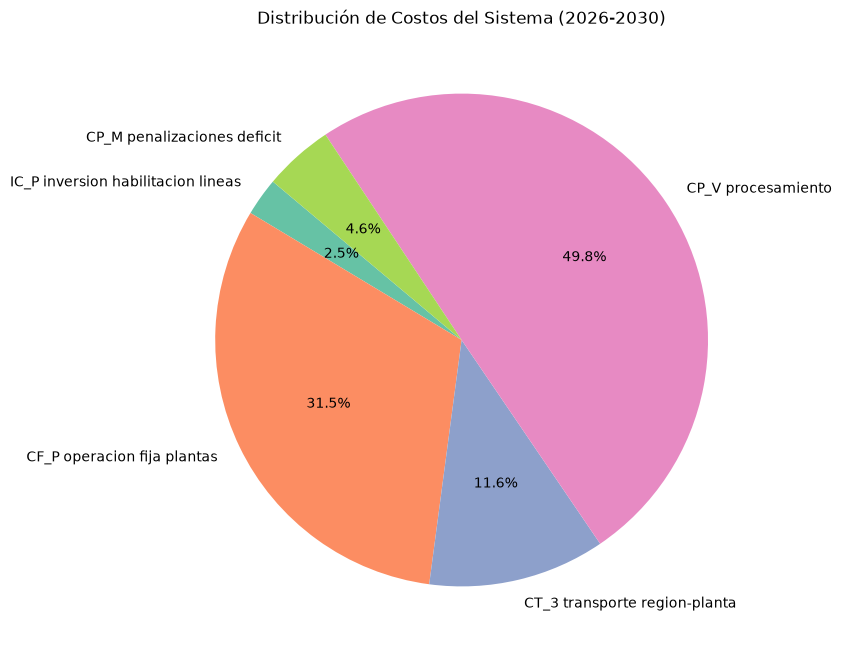
\includegraphics[width=\textwidth]{grafico_costos.png}
    \caption{Distribución porcentual de costos del sistema.}
    \label{fig:grafico_costos}
\end{minipage}
\hfill
\begin{minipage}[t]{0.48\textwidth}
    \centering
    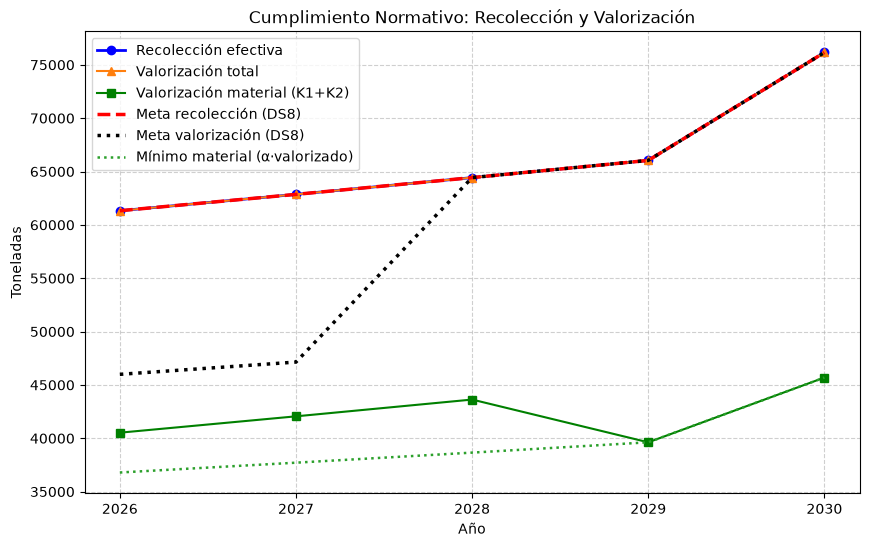
\includegraphics[width=\textwidth]{grafico_metas.png}
    \caption{Recolección, valorización y metas DS8 por año.}
    \label{fig:grafico_metas}
\end{minipage}
\vspace{-3mm}
\end{figure}
\begin{table}[H]
\centering
\caption{Desglose del valor óptimo de la función objetivo por componente (2026--2030).}
\label{tab:costos_fo}
\small
\setlength{\tabcolsep}{4pt}
\begin{tabularx}{\linewidth}{@{}>{\raggedright\arraybackslash}Xrrr@{}}
\hline
\textbf{Componente de costo} & \shortstack{\textbf{Costo}\\\textbf{[M\$]}} & \shortstack{\textbf{Costo}\\\textbf{[MM\$]}} & \shortstack{\textbf{Participación}\\\textbf{[\%]}} \\
\hline
Procesamiento variable en plantas ($CP\_V$) & $40.811.228,65$ & $40.811,23$ & $49,82\%$ \\
Operación fija anual de plantas ($CF\_P$) & $25.822.500,00$ & $25.822,50$ & $31,52\%$ \\
Transporte directo región--planta ($CT\_3$) & $9.506.913,23$ & $9.506,91$ & $11,60\%$ \\
Penalizaciones por déficit normativo ($CP\_M$) & $3.741.964,43$ & $3.741,96$ & $4,57\%$ \\
Inversión en habilitación de líneas ($IC\_P$) & $2.040.000,00$ & $2.040,00$ & $2,49\%$ \\
Habilitación, operación fija, flete y acopio en centros & $0,00$ & $0,00$ & $0,00\%$ \\
\hline
\textbf{Total Función Objetivo ($Z^{*}$)} & \textbf{81.922.606,31} & \textbf{81.922,61} & \textbf{100,00\%} \\
\hline
\end{tabularx}
\end{table}

Un hallazgo estratégico para \textit{Valora Más} es que la solución óptima no abre centros de acopio ($y_{ct}=0\;\forall c,t$) y envía el 100\% del flujo directo de región a planta ($z_{rpt}$). El ahorro de $8\%$ en la tarifa del tramo T2 no compensa la tarifa del tramo T1, los costos fijos de acopio ($185.000$ a $1.156.250\text{ M\$/año}$) ni su inversión ($45.000$ a $234.000\text{ M\$}$). Como toda tonelada recolectada se valoriza el mismo año, en 2026 y 2027 la valorización alcanza el $80\%$, sobre el $60\%$ exigido: es más barato procesar ese excedente en plantas con capacidad disponible que habilitar centros solo para guardar inventario.

Con el cobro por viaje, el tipo de camión pasa a ser una decisión real. El 99,6\% de los viajes se hace en camiones de 25 t, y los de 10 y 15 t (49 viajes en el quinquenio) se usan solo para llevar los saldos que no completan un camión grande; por ejemplo, Magallanes envía 540 t en 2026 con 21 viajes de 25 t y uno de 15 t. Así, la ocupación media de la flota es de $99,99\%$. El modelo incluso ajusta las toneladas recolectadas a camiones completos: Arica envía 600 t (24 viajes de 25 t) en 2026, 2029 y 2030, aunque podría recolectar algo más.

\subsection{Plan de Expansión de Plantas, Tecnologías y Flujos Logísticos}

La Tabla~\ref{tab:balance_anual} y la Figura~\ref{fig:grafico_metas} resumen los indicadores anuales; la Tabla~\ref{tab:plantas_uso} detalla el plan de habilitación de líneas y su utilización.

\begin{table}[H]
\centering
\caption{Balance anual de generación, recolección, valorización y viajes de flota (2026--2030).}
\label{tab:balance_anual}
\small
\setlength{\tabcolsep}{3pt}
\begin{tabularx}{\linewidth}{@{}>{\raggedright\arraybackslash}Xrrrrrr@{}}
\hline
\textbf{Indicador} & \textbf{2026} & \textbf{2027} & \textbf{2028} & \textbf{2029} & \textbf{2030} & \textbf{Total} \\
\hline
Generación [ton] & $76.658,1$ & $78.574,6$ & $80.538,7$ & $82.552,2$ & $84.616,1$ & $402.939,7$ \\
Meta recolección & $80\%$ & $80\%$ & $80\%$ & $80\%$ & $90\%$ & -- \\
Rec./Val. [ton] & $61.326,48$ & $62.859,68$ & $64.430,96$ & $66.041,76$ & $76.154,49$ & $330.813,37$ \\
Rec./Val. [\%] & $80,0\%$ & $80,0\%$ & $80,0\%$ & $80,0\%$ & $90,0\%$ & $82,1\%$ \\
Val. material [ton] & $40.526,48$ & $42.059,68$ & $43.630,96$ & $39.625,06$ & $45.692,69$ & $211.534,87$ \\
Material [\%] & $66,1\%$ & $66,9\%$ & $67,7\%$ & $60,0\%$ & $60,0\%$ & $63,9\%$ \\
Déficit $d^{Q}$ [ton] & $657,75$ & $674,39$ & $691,07$ & $708,30$ & $726,00$ & $3.457,51$ \\
Viajes 10t / 15t & $5\,/\,2$ & $5\,/\,4$ & $5\,/\,8$ & $5\,/\,7$ & $2\,/\,6$ & $22\,/\,27$ \\
Viajes 25t & $2.450$ & $2.510$ & $2.571$ & $2.636$ & $3.042$ & $13.209$ \\
Ocupación flota [\%] & $99,99\%$ & $100,0\%$ & $99,98\%$ & $99,98\%$ & $99,99\%$ & $99,99\%$ \\
\hline
\end{tabularx}
\end{table}

\begin{table}[H]
\centering
\caption{Plan de habilitación de plantas y toneladas valorizadas por línea tecnológica [ton/año].}
\label{tab:plantas_uso}
\small
\setlength{\tabcolsep}{3pt}
\begin{tabular*}{\linewidth}{@{\extracolsep{\fill}}llrrrrrr@{}}
\hline
\textbf{Planta} & \textbf{Tec. (Cat.)} & \textbf{Cap. [ton]} & \textbf{2026} & \textbf{2027} & \textbf{2028} & \textbf{2029} & \textbf{2030} \\
\hline
P02 Antofagasta & K2 (Mat.) & $11.000$ & $7.526,8$ & $9.059,7$ & $10.631,0$ & $6.627,2$ & $5.393,3$ \\
P04 Valparaíso & K3 (Ene.) & $10.400$ & -- & -- & -- & $7.640,0$ & $9.679,3$ \\
P05 RM Norte & K2 (Mat.) & $22.000$ & $22.000,0$ & $22.000,0$ & $22.000,0$ & $21.998,3$ & $22.000,0$ \\
P05 RM Norte & K3 (Ene.) & $10.400$ & $10.400,0$ & $10.400,0$ & $10.400,0$ & $8.376,7$ & $10.384,6$ \\
P07 O'Higgins & K2 (Mat.) & $11.000$ & $10.999,7$ & $11.000,0$ & $11.000,0$ & $10.999,6$ & $11.000,0$ \\
P09 Biobío & K3 (Ene.) & $10.400$ & $10.400,0$ & $10.400,0$ & $10.400,0$ & $10.400,0$ & $10.397,9$ \\
P10 Los Lagos & K2 (Mat.) & $11.000$ & -- & -- & -- & -- & $7.299,4$ \\
\hline
\end{tabular*}
\par\smallskip
{\footnotesize K2: trituración material; K3: coprocesamiento energético.}
\end{table}

El modelo selecciona solo dos tecnologías: trituración mecánica (K2, $145\text{ M\$/ton}$) para cumplir la cuota del 60\% de valorización material, y coprocesamiento cementero (K3, $85\text{ M\$/ton}$) para el complemento energético, descartando el recauchaje (K1, $2.650\text{ M\$/ton}$) y la pirólisis (K4, $280\text{ M\$/ton}$). En 2026 se habilitan 5 líneas base: K2 en P02 Antofagasta, K2 y K3 en P05 RM Norte, K2 en P07 O'Higgins y K3 en P09 Biobío ($64.800\text{ ton/año}$), que en la zona central y Biobío operan prácticamente a plena capacidad. En 2029, cuando la meta supera esa capacidad, se habilita K3 en P04 Valparaíso y la proporción material baja exactamente al mínimo de $60\%$. Ante el salto al $90\%$ en 2030 se habilita K2 en P10 Los Lagos, que recibe los flujos de Los Ríos, Los Lagos, Aysén y Magallanes y acorta los fletes de la macrozona sur-austral. Como la zona central está llena, el modelo envía NFU largas distancias: Coquimbo despacha hasta $3.490\text{ ton/año}$ a P02 Antofagasta (890 km), su séptima planta más cercana; la capacidad disponible pesa más que la distancia.

En las regiones extremas, Arica y Parinacota envía entre $600$ y $1.115\text{ ton/año}$ a P02 Antofagasta, y Aysén ($385$ a $425\text{ ton/año}$) y Magallanes ($540$ a $600\text{ ton/año}$) a P09 Biobío entre 2026 y 2029 y a P10 Los Lagos en 2030. El tope de flota (R13) no se activa, pero tiene poca holgura: en Magallanes los viajes a Biobío usan hasta el $79,7\%$ de los camión-días del camión de 25 t, y en Arica el $67,7\%$.

\section{Validación y Optimalidad}

\subsection{Certificación de Optimalidad y Factibilidad Matemática}

La solución cuenta con certificación de optimalidad ($\text{Status = OPTIMAL}$, código 2 de Gurobi): la mejor solución entera ($Z^{*} = 81.922.606,31\text{ M\$}$) y la cota inferior ($81.918.527,88\text{ M\$}$) difieren en $0,005\%$, bajo la tolerancia de $0,01\%$. Las desigualdades válidas R14 fueron clave: elevaron la relajación lineal del nodo raíz de $77.085.490$ a $78.549.060\text{ M\$}$. Sin ellas, la misma instancia alcanzó el límite de $1.800\text{ s}$ con un gap de $0,96\%$, aunque con la misma solución. Esa solución aparece a los $\sim$300 s en ambas corridas y no cambia después, por lo que un computador más lento obtendría el mismo $Z^{*}$ aunque no alcanzara a certificarlo.

La factibilidad y el balance de masa se verifican con residuo nulo (menor a $10^{-9}$ ton) en todos los años: sin inventario en centros ($s_{oct}=0$), las $330.813,37\text{ ton}$ recolectadas igualan las valorizadas. Se cumplen las capacidades de plantas (R6), el límite de líneas por complejo (R6c, máximo 2 activas en P05 frente a 4), la permanencia (R10), la capacidad vehicular (R0), con $13.258$ viajes que transportan $330.813,37$ de $330.850\text{ ton}$ contratadas, y el tope de flota (R13), con un uso máximo de $79,7\%$.

\subsection{Coherencia Operativa y Análisis del Déficit en Atacama}

Los resultados son coherentes con los costos, capacidades y disponibilidades estimadas de la instancia, considerando las siguientes limitaciones:

\textbf{Racionalidad económica en la selección tecnológica y logística}: El modelo usa el coprocesamiento (K3) hasta el tope que permite R12 ($40\%$ de lo valorizado en 2029--2030), por su menor costo fijo y variable, y completa el $60\%$ material solo con trituración (K2). La apertura de P04 Valparaíso en 2029 y P10 Los Lagos en 2030 responde al agotamiento de la capacidad inicial ($64.800\text{ ton/año}$) y a la conveniencia de acercar la trituración a la zona sur-austral cuando la meta sube al $90\%$.

\textbf{Interpretación del déficit en Atacama ($d^{Q}_{\text{R04},t}>0$)}: Los déficits nacionales son nulos ($d^{R}_{t}=d^{V}_{t}=0\;\forall t$). Atacama acumula un déficit de $3.457,49\text{ ton}$ porque su participación estimada en el parque vehicular ($1,64\%$) es menor que su cuota ($2,50\%$): en 2026 la cuota de $1.916,5\text{ ton}$ supera en $657,8\text{ ton}$ la disponibilidad de $1.258,7\text{ ton}$, que se recolecta completa. El único otro déficit es de $0,02\text{ ton}$ en Magallanes en 2027: penalizarlo cuesta $24\text{ M\$}$, mientras que un viaje extra de 10 t a Biobío costaría $2.223\text{ M\$}$, así que el modelo prefiere la penalización. La penalización total es de $3.741.964,43\text{ M\$}$.

El déficit de Atacama depende de la estimación y no prueba escasez física real. La explicación mediante flujos de faenas y contratistas omitidos es una hipótesis. La solución admite incumplimiento penalizado y cobertura por origen; no certifica cumplimiento normativo total.


\clearpage
\section{Anexos}
\begingroup
\small
\sloppy
\subsection*{Anexo A: Diccionario de Datos de \texttt{datos.xlsx}}
El archivo principal de parámetros, \texttt{datos.xlsx}, consolida toda la información operacional, financiera y normativa del problema. A continuación, se describen las hojas principales y sus parámetros de entrada:


\textbf{Hoja \texttt{Metas\_\allowbreak DS8}:} Define las metas anuales de recolección y valorización exigidas por la Ley REP (DS8), la cuota mínima de valorización material ($\alpha_t^M=0,60$) y los coeficientes económicos aproximados por tonelada de déficit ($\mu_t^R, \mu_t^V, \mu_t^Q$).\\
{\raggedright \textit{Columnas:} \texttt{Anio\_\allowbreak t, Meta\_\allowbreak Recoleccion\_\allowbreak mR, Meta\_\allowbreak Valorizacion\_\allowbreak mV, Cuota\_\allowbreak Min\_\allowbreak Material\_\allowbreak alphaM, Penalizacion\_\allowbreak muR, Penalizacion\_\allowbreak muV, Penalizacion\_\allowbreak muQ, Fuente\_\allowbreak Normativa}.\par}

\textbf{Hoja \texttt{Regiones\_\allowbreak Generacion}:} Establece la generación anual proyectada de NFU (toneladas) por cada una de las 16 regiones de Chile y la cuota regional tomada del DS8 y aplicada como cobertura por origen en R9.\\
{\raggedright \textit{Columnas:} \texttt{ID\_\allowbreak Region, Nombre\_\allowbreak Region, Cuota\_\allowbreak DS8\_\allowbreak qr, Gen\_\allowbreak 2026} a \texttt{Gen\_\allowbreak 2030, Fuente\_\allowbreak Base}.\par}

\textbf{Hoja \texttt{Centros\_\allowbreak Acopio}:} Detalla las capacidades operativas (recepción y despacho), los costos fijos y de habilitación, y los límites sanitarios de inventario de los 16 centros de acopio candidatos.\\
{\raggedright \textit{Columnas:} \texttt{ID\_\allowbreak Centro, Nombre\_\allowbreak Centro, ID\_\allowbreak Region\_\allowbreak Ubicacion, Cap\_\allowbreak Recepcion\_\allowbreak aC, Cap\_\allowbreak Despacho\_\allowbreak bC, Limite\_\allowbreak Sanitario\_\allowbreak sM, Inv\_\allowbreak Inicial\_\allowbreak s0, Costo\_\allowbreak Fijo\_\allowbreak Anual\_\allowbreak cF, Costo\_\allowbreak Almacenaje\_\allowbreak h, Inversion\_\allowbreak Habilitacion\_\allowbreak iC}.\par}

\textbf{Hoja \texttt{Plantas\_\allowbreak Tecnologias}:} Determina los sitios candidatos para las plantas de valorización, indicando mediante el parámetro binario de factibilidad ($e_{pk}$) qué tecnologías pueden instalarse en cada una, sus capacidades anuales, costos fijos e inversión de habilitación inicial.\\
{\raggedright \textit{Columnas:} \texttt{ID\_\allowbreak Planta, Nombre\_\allowbreak Planta, ID\_\allowbreak Region\_\allowbreak Ubicacion, ID\_\allowbreak Tecnologia, Max\_\allowbreak Lineas\_\allowbreak nP, Factibilidad\_\allowbreak epk, Cap\_\allowbreak Efectiva\_\allowbreak aP, Costo\_\allowbreak Fijo\_\allowbreak cP, Inversion\_\allowbreak Habilitacion\_\allowbreak iP}.\par}

\textbf{Hoja \texttt{Tecnologias\_\allowbreak Costos}:} Clasifica las alternativas tecnológicas (ej. Recauchaje, Trituración mecánica, Coprocesamiento) en las categorías estipuladas en el DS8, indicando su costo variable operativo por tonelada tratada.\\
{\raggedright \textit{Columnas:} \texttt{ID\_\allowbreak Tecnologia, Nombre\_\allowbreak Tecnologia, Subconjunto\_\allowbreak DS8, Costo\_\allowbreak Variable\_\allowbreak cV}.\par}

\textbf{Hoja \texttt{Costos\_\allowbreak Transporte}:} Matriz que define las distancias (en kilómetros) y los costos logísticos de transporte por tonelada para los distintos tramos de la red (región-centro, centro-planta, región-planta).\\
{\raggedright \textit{Columnas:} \texttt{Tipo\_\allowbreak Tramo, Nodo\_\allowbreak Origen, Nodo\_\allowbreak Destino, Distancia\_\allowbreak Ruta, Costo\_\allowbreak Unitario}.\par}

\textbf{Hojas \texttt{Flota\_\allowbreak Camiones}, \texttt{Parametros\_\allowbreak Flota} y \texttt{Tope\_\allowbreak Flota}:} Capacidad por viaje y factor tarifario de cada camión ($q^V_u, f^V_u$), parámetros para calcular los camión-días por viaje ($v, H, t^{CD}, D$) y camiones disponibles por región extrema ($K_{ru}$), cada uno con su fuente.\\
{\raggedright \textit{Columnas:} \texttt{ID\_\allowbreak Camion, Cap\_\allowbreak Viaje\_\allowbreak qV, Factor\_\allowbreak Tarifario\_\allowbreak fV}; \texttt{Parametro, Valor, Unidad}; \texttt{ID\_\allowbreak Region, Camiones\_\allowbreak Camion\_\allowbreak 10t} a \texttt{Camiones\_\allowbreak Camion\_\allowbreak 25t}.\par}

\textbf{Hojas de Metadatos (\texttt{MD\_\allowbreak Bloque1} a \texttt{MD\_\allowbreak Bloque6}):} Repositorio de respaldo de las fuentes oficiales (INE, SII, MMA) y proyecciones. Documentan de dónde se extrajo cada costo y volumen garantizando la trazabilidad de los supuestos financieros y de infraestructura.


\endgroup
\newpage
% Se conservan las referencias del informe original.
\IfFileExists{referencias.bib}{%
\bibliographystyle{plain}
\bibliography{referencias}
}{%
\begin{thebibliography}{17}
\bibitem{bodegas2026}
Agenda Logística. Bodegas flex ganan terreno: absorción neta crece 244 \% y vacancia baja 38 \%, septiembre 2026. Datos del informe de Cushman \& Wakefield. \url{https://assets.cushmanwakefield.com/-/media/cw/americas/chile/insights/2026/informe-bodegas-flex-s1-2026.pdf}

\bibitem{amphos2017}
Amphos 21. Diagnóstico de sustentabilidad de neumáticos fuera de uso. Technical report, Ministerio del Medio Ambiente de Chile, 2017. \url{https://economiacircular.mma.gob.cl/wp-content/uploads/2019/06/8.-Diagnostico-de-sustentabilidad-de-NFU.-Amphos21-2017.pdf}

\bibitem{arrigoni}
Arrigoni Ambiental NFU. Quiénes somos: valorización de neumáticos fuera de uso mediante pirólisis. Sitio web oficial de Arrigoni Ambiental NFU. Consultado en octubre de 2026. \url{https://arrigoniambientalnfu.cl/servicios/planta-de-reciclaje-nfu-por-pirolisis/}

\bibitem{leyrep20920}
Biblioteca del Congreso Nacional de Chile. Ley Nº 20.920: Establece marco para la gestión de residuos, la responsabilidad extendida del productor y fomento al reciclaje. Ley Chile, 2016. \url{https://www.bcn.cl/leychile/navegar?idNorma=1090894}

\bibitem{dt2025}
Biblioteca del Congreso Nacional de Chile. Código del Trabajo (DFL N.º 1 de 2002), artículo 25 bis: jornada de choferes de transporte de carga interurbana. Ley Chile. \url{https://www.bcn.cl/leychile/navegar?idNorma=207436}

\bibitem{induambiente2021}
InduAmbiente. A partir de hoy rigen las metas de recolección y valorización para neumáticos. InduAmbiente, enero 2021. \url{https://www.induambiente.com/actualidad/noticias/a-partir-de-hoy-rigen-las-metas-de-recoleccion-y-valorizacion-para-neumaticos}

\bibitem{INE2025}
Instituto Nacional de Estadísticas. Informe anual de estadísticas del medio ambiente 2025. Technical report, Instituto Nacional de Estadísticas de Chile, 2025. Cuadro 11.2.2, página 133. \url{https://www.ine.gob.cl/docs/default-source/variables-basicas-ambientales/publicaciones-y-anuarios/informe-anual-de-medio-ambiente/informe-anual-de-estadisticas-del-medio-ambiente-2025.pdf}

\bibitem{kyklos2026}
Kyklos. Capacidad instalada y proyección para la valorización de NFU. Technical report, Kyklos, por encargo de Valora Más, 2026. Estudio presentado en seminario web y citado en País Circular, 13 de julio de 2026. \url{https://www.paiscircular.cl/economia-circular/estudio-evidencia-cuello-de-botella-en-la-demanda-de-los-subproductos-de-la-valorizacion-de-neumaticos-fuera-de-uso/}

\bibitem{melon}
Melón S.A. Coprocesamiento melón: Un círculo de valor sostenible. Caso empresarial publicado en la plataforma Conecta de Pacto Global Chile. Consultado en octubre de 2026. \url{https://conecta.pactoglobal.cl/casos-de-empresas/coprocesamiento-melon-un-circulo-de-valor-sostenible/}

\bibitem{DS8}
Ministerio del Medio Ambiente de Chile. Decreto Supremo Nº 8: Establece metas de recolección y valorización, y otras obligaciones asociadas, a los productores de neumáticos. Technical report, Ministerio del Medio Ambiente, 2021. Publicado en el Diario Oficial el 20 de enero de 2021. \url{https://www.bcn.cl/leychile/navegar?idNorma=1154847}

\bibitem{bases2024}
Neuvol. Bases de licitación: Compra o cobro de NU y NFU enteros con el fin de valorizarlos efectivamente. Portal Neuvol, febrero 2024. \url{https://portal.neuvol.cl/_entity/sharepointdocumentlocation/e815b512-b3d5-ee11-a81c-002248df2318/0bd39e64-31e0-ec11-bb3d-000d3a88dfb9?file=2024_02_27_BASES\%20LICITACIO\%CC\%81N\%20VALORIZACIO\%CC\%81N.pdf}

\bibitem{paiscircular2025}
País Circular. Nathalia Silva, gerenta general de Valora Más: “Este 2025 estamos logrando la cobertura en todos los territorios del país”. País Circular, 2025. \url{https://www.paiscircular.cl/economia-circular/nathalia-silva-de-valora-mas-este-2025-estamos-logrando-la-cobertura-en-todos-los-territorios/}

\bibitem{polambiente}
Polambiente. Nosotros: valorización de neumáticos fuera de uso. Sitio web oficial de Polambiente. Consultado en octubre de 2026. \url{https://polambiente.cl/nosotros/}

\bibitem{rivera2023}
Luis Rivera Venegas. Planta de reciclaje de neumáticos fuera de uso de minería a través de pirólisis. Master’s thesis, Universidad de Chile, 2023. Parte I, páginas 11 y 49. \url{https://repositorio.uchile.cl/bitstream/handle/2250/202400/Tesis\%20-\%20Luis\%20Rivera\%20Venegas\%20-\%20Parte\%20I.pdf}

\bibitem{sii2026}
Servicio de Impuestos Internos. Valores de la UTM, UTA e IPC 2026. SII, 2026. Consultado en octubre de 2026. \url{https://www.sii.cl/valores_y_fechas/utm/utm2026.htm}

\bibitem{steer2020}
Steer. Actualización de modelo de costos de transporte de carga para el análisis de costos logísticos, del observatorio logístico. Technical report, Subsecretaría de Transportes de Chile, 2020. Tabla 4.44, página 75. \url{https://www.observatoriologistico.cl/sites/default/files/2024-06/eaaaa88d-8a05-456d-8976-3e0e09fa60ba.pdf}

\bibitem{paiscircular2026}
Fabiola Venegas Órdenes. Nathalia Silva, de Valora Más, advierte que la falta de demanda para los neumáticos reciclados “es una bomba de tiempo” para la sostenibilidad de la REP. País Circular, mayo 2026. \url{https://www.paiscircular.cl/economia-circular/nathalia-silva-de-valora-mas-advierte-que-la-falta-de-demanda-para-los-neumaticos-reciclados-es-una-bomba-de-tiempo-para-la-sostenibilidad-de-la-ley-rep/}

\end{thebibliography}
}

\end{document} 